
%(BEGIN_QUESTION)
% Copyright 2010, Tony R. Kuphaldt, released under the Creative Commons Attribution License (v 1.0)
% This means you may do almost anything with this work of mine, so long as you give me proper credit

Noe er galt med denne ventilstyrekretsen. Når operatøren trykker ``open''-trykknappen, viser ventilens posisjonslamper fortsatt at den er lukket (grønn lampe på, rød lampe av):

$$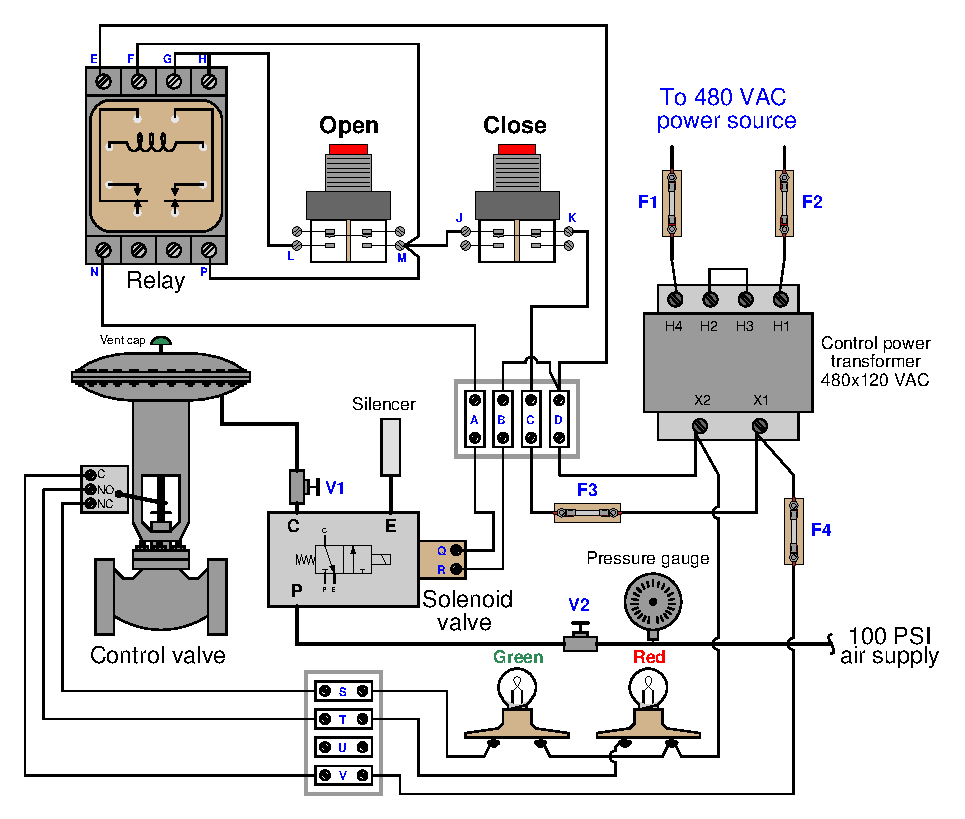
\includegraphics[width=15.5cm]{i01564x01.eps}$$

Bestem diagnostisk verdi av hver av følgende tester. Anta bare én feil i systemet, inkludert en enkelt komponent eller en enkelt ledning/kabel/rørforbindelse mellom komponenter. Hvis en foreslått test kan gi ny informasjon som hjelper deg å identifisere plassering og/eller type feil, marker ``ja''. Hvis en foreslått test ikke vil avsløre noe relevant for identifisering av feilen (allerede utledbart fra målinger og symptomer så langt), marker ``nei''.

% No blank lines allowed between lines of an \halign structure!
% I use comments (%) instead, so that TeX doesn't choke.

$$\vbox{\offinterlineskip
\halign{\strut
\vrule \quad\hfil # \ \hfil & 
\vrule \quad\hfil # \ \hfil & 
\vrule \quad\hfil # \ \hfil \vrule \cr
\noalign{\hrule}
%
% First row
{\bf Diagnostisk test} & {\bf Ja} & {\bf Nei} \cr
%
\noalign{\hrule}
%
% Another row
Mål AC-spenning over sikring F1 &  &  \cr
%
\noalign{\hrule}
%
% Another row
Mål AC-spenning over sikring F3 &  &  \cr
%
\noalign{\hrule}
%
% Another row
Mål AC-spenning over magnetspolen med ``Open''-knappen trykket inn &  &  \cr
%
\noalign{\hrule}
%
% Another row
Mål AC-spenning over magnetspolen med ``Closed''-knappen trykket inn &  &  \cr
%
\noalign{\hrule}
%
% Another row
Mål AC-spenning mellom terminal X2 og T med ``Open''-knappen trykket inn &  &  \cr
%
\noalign{\hrule}
%
% Another row
Mål AC-spenning mellom terminal L og D med ``Open''-knappen trykket inn &  &  \cr
%
\noalign{\hrule}
%
% Another row
Sjekk luftforsyningstrykk (se på manometer) &  &  \cr
%
\noalign{\hrule}
} % End of \halign 
}$$ % End of \vbox

\vfil 

\underbar{file i01564}
\eject
%(END_QUESTION)





%(BEGIN_ANSWER)

Dette er et vurdert spørsmål -- ingen svar eller hint gitt!

%(END_ANSWER)





%(BEGIN_NOTES)

En god problemløsningsstrategi i slike tilfeller, der vi må vurdere nytten av ulike diagnostiske tester, er først å avgjøre hva som kan være feilet i kretsen, og hva vi vet er i orden. Først da kan vi avgjøre om en bestemt test vil gi ny informasjon om feilen (kriteriet for en gyldig diagnostisk test).

For eksempel viser den grønne lampen at kretsen har spenning. Det betyr blant annet at sikringene F1, F2 og F4 er i orden. Dermed er enhver måling av AC-spenning over F1 en dårlig test, fordi vi allerede vet fra grønnlampens lys at F1 må være i orden og derfor får (nesten) null volt spenningsfall.

% No blank lines allowed between lines of an \halign structure!
% I use comments (%) instead, so that TeX doesn't choke.

$$\vbox{\offinterlineskip
\halign{\strut
\vrule \quad\hfil # \ \hfil & 
\vrule \quad\hfil # \ \hfil & 
\vrule \quad\hfil # \ \hfil \vrule \cr
\noalign{\hrule}
%
% First row
{\bf Diagnostisk test} & {\bf Ja} & {\bf Nei} \cr
%
\noalign{\hrule}
%
% Another row
Mål AC-spenning over sikring F1 med ``Closed''-knappen trykket inn &  & $\surd$ \cr
%
\noalign{\hrule}
%
% Another row
Mål AC-spenning over sikring F3 med ``Closed''-knappen trykket inn & $\surd$ &  \cr
%
\noalign{\hrule}
%
% Another row
Mål AC-spenning over magnetspolen med ``Open''-knappen trykket inn & $\surd$ &  \cr
%
\noalign{\hrule}
%
% Another row
Mål AC-spenning over magnetspolen med ``Closed''-knappen trykket inn &  & $\surd$ \cr
%
\noalign{\hrule}
%
% Another row
Mål AC-spenning mellom terminal X2 og T med ``Open''-knappen trykket inn &  & $\surd$ \cr
%
\noalign{\hrule}
%
% Another row
Mål AC-spenning mellom terminal L og D med ``Open''-knappen trykket inn & $\surd$ &  \cr
%
\noalign{\hrule}
%
% Another row
Sjekk luftforsyningstrykk (se på manometer) & $\surd$ &  \cr
%
\noalign{\hrule}
} % End of \halign 
}$$ % End of \vbox

\vskip 20pt \vbox{\hrule \hbox{\strut \vrule{} {\bf Virtuell feilsøking} \vrule} \hrule}

Denne oppgaven egner seg godt som en ``Virtuell feilsøking''-øvelse. Når du presenterer diagrammet for studentene, ser du først for deg en bestemt feil i systemet. Deretter presenterer du ett eller flere symptomer på feilen (noe en operatør eller annen bruker av systemet kan observere). Studentene foreslår så ulike diagnostiske tester for å identifisere type og plassering av feilen, som om de var teknikere som feilsøker problemet. Din oppgave er å fortelle hva resultatet ville blitt av hver foreslåtte test, og dokumentere resultatene slik at alle studentene kan se dem.

Under og etter øvelsen er det nyttig å stille oppfølgingsspørsmål som:

\begin{itemize}
\item{} Hva forteller resultatet av den siste diagnostiske testen om feilen?
\item{} Anta at resultatene av den siste diagnostiske testen var annerledes. Hva ville det resultatet da fortelle om feilen?
\item{} Er den siste diagnostiske testen den beste vi kunne utført?
\item{} Hva ville vært den ideelle rekkefølgen av tester for å diagnostisere problemet med færrest mulige trinn?
\end{itemize}


%INDEX% Troubleshooting review: electric circuit diagnostic test usefulness

%(END_NOTES)

